
\documentclass[]{article}
\usepackage{graphicx}
\usepackage{hyperref}
%opening
\title{Péndulo invertido}
\author{Marcos Fontenlos Ferreiro}

\begin{document}
 
\maketitle

\section{Propuesta}
\paragraph{}
Como parte de la asignatura de teoría de control se nos propuso crear un dispositivo que fuese capaz de mantener el equilibrio sobre dos ruedas empleando un control PID. En conjunto, tuvimos que diseñar nuestra propia PCB para la instalación del hardware, la base sobre la que está montada el dispositivo y el software de control con el que calibraremos el PID para obtener la estabilidad deseada.

\section{Hardware}
\paragraph{}
Para el montaje de nuestro dispositivo tuvimos que elegir los componentes electrónicos para el funcionamiento. En nuestro caso para darle autonomía y economía al proyecto nos decidimos por emplear un Esp32, un microcontrolador económico y versátil que , además contiene un módulo Wi-fi que nos permitirá controlar el dispositivo desde una aplicación externa. 

\paragraph{}
Alrededor de este microcontrolador montaremos un giroscopio, el MPU6050, para determina la orientacion de nuestro dispositivo, y también gestionaremos dos motores de corriente continua por medio de un driver, el TB6612FNG. Este driver nos permitirá aislar la parte de potencia de los motores, que será suministrada por un portapilas (4xAA)
, de la parte de control, que será completamente gestionada por nuestro microcontrolador.
\paragraph{}
Para facilitar las conexiones entre los motores, el portapilas y la PCB soldamos unos pequeños conectores a la placa y a los terminales de los otros elementos para limpieza y seguridad. Para comunicar nuestros componentes de la PCB utilizamos pines GPIO para el driver y el protocolo I2C para el sensor.
\paragraph{}
En síntesis necesitaremos entonces, microcontrolador (ESP32), sensor (giroscopio MPU6050) y driver (TB6612FNG). Estos componentes deberán ser integrados en la PCB con su respectiva alimentación. Esta alimentación serán 6V, que llegarán íntegros al driver. Por otro lado, como al microcontrolador solo pueden llegar 5V, utilizamos un regulador de voltaje, el LM7605 junto con un par de condensadores para limitar la caída de tensión. 


\begin{figure}[!h]
	\centering
	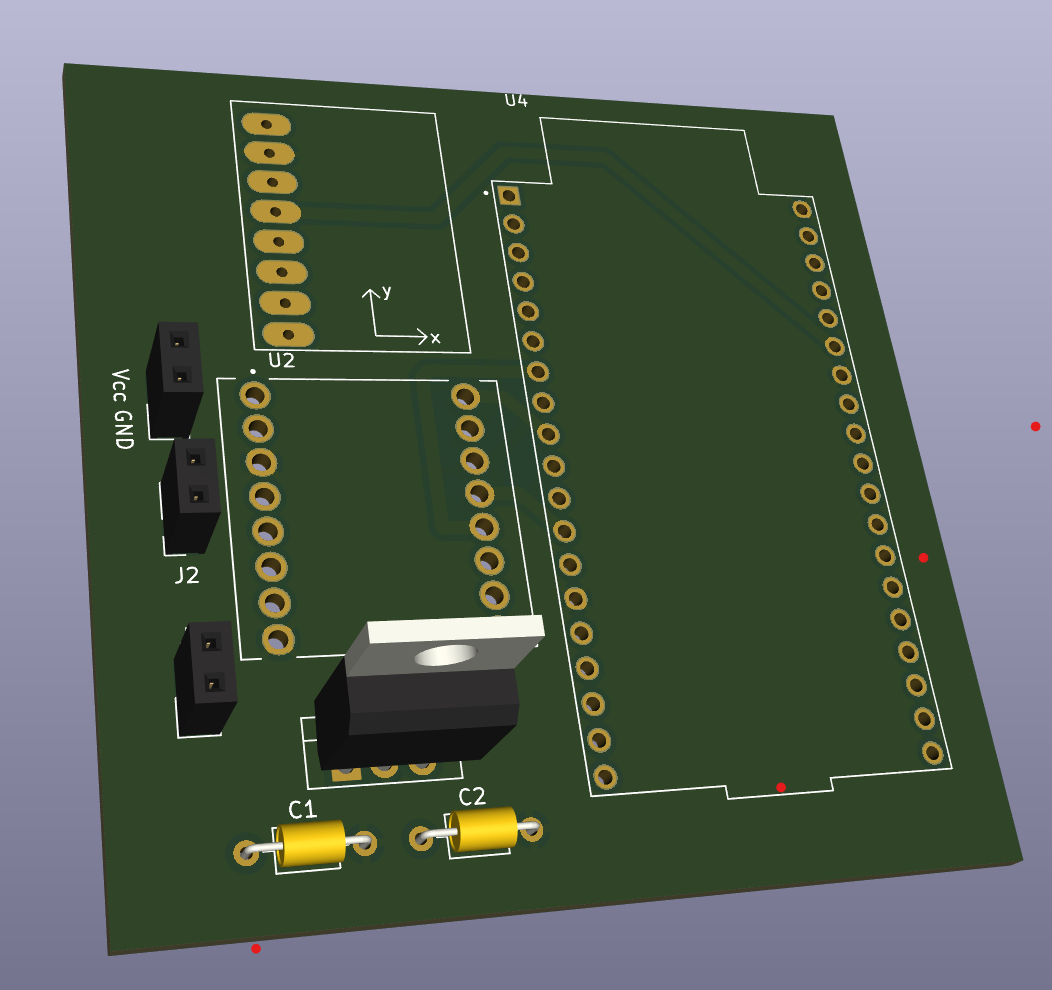
\includegraphics[width=0.5\linewidth]{PCB}
	\caption{}
	\label{fig:pcb}
\end{figure}

\begin{figure}[!h]
	\centering
	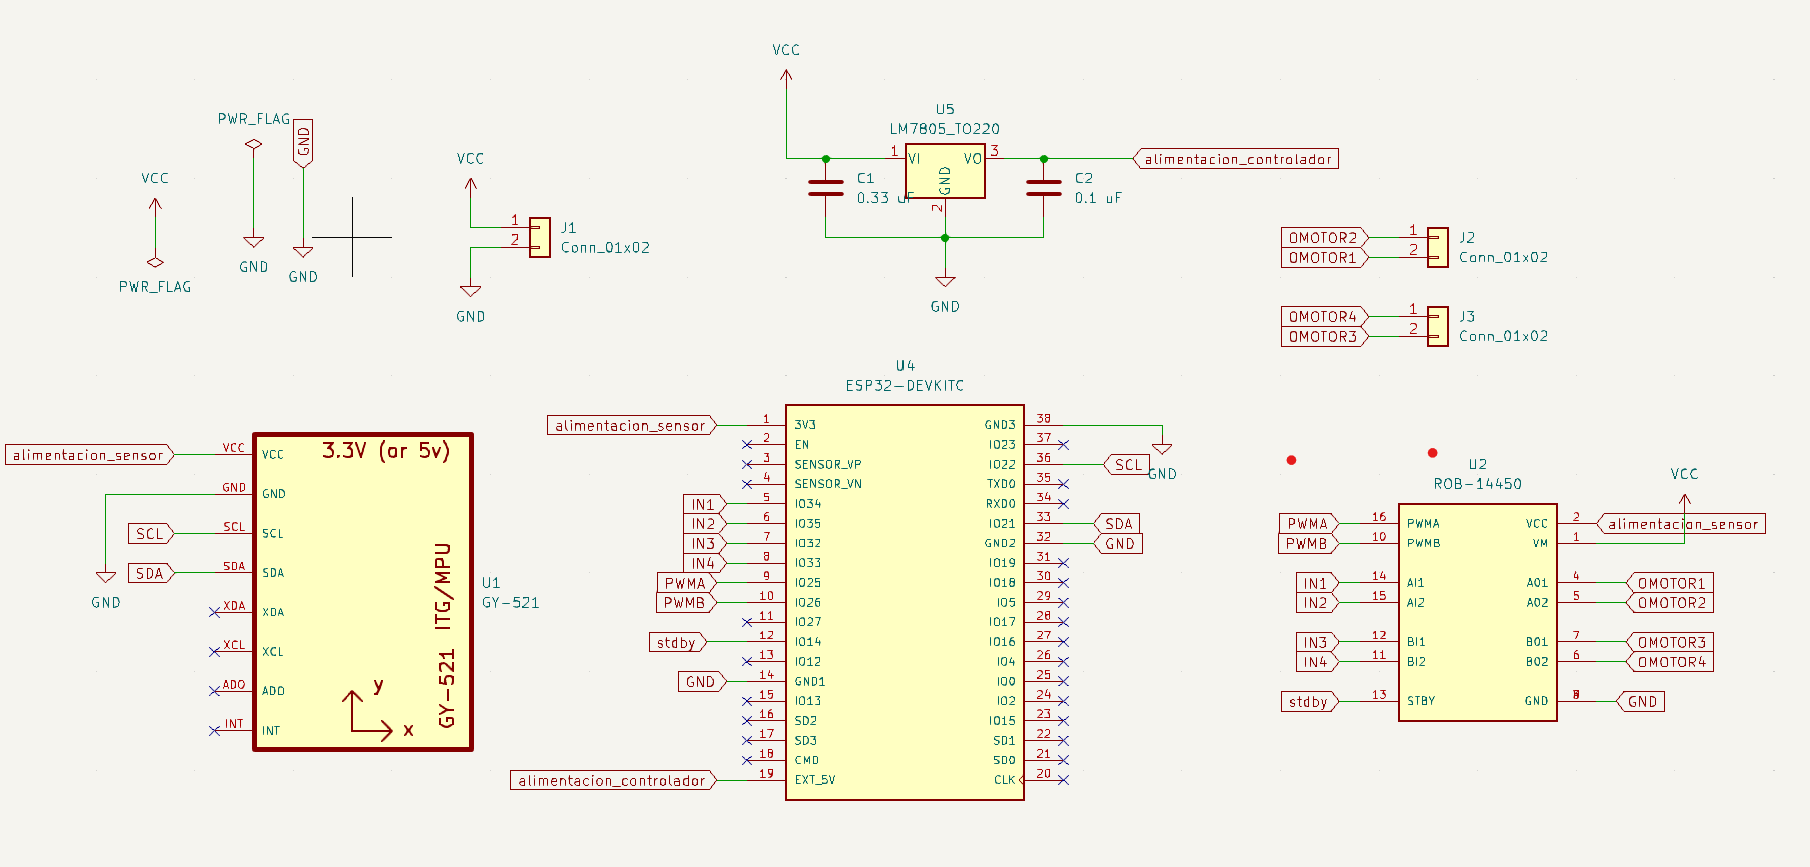
\includegraphics[width=1\linewidth]{PCB1}
	\caption{}
	\label{fig:pcb1}
\end{figure}
\paragraph{}
\paragraph{}
Con la PCB diseñada y  los componentes soldados, nos encontramos con diversas problemáticas. La primera de ellas, en la conexión entre driver y ESP32, estábamos utilizando unos pines GPIO que solo permitían input, y no output, por lo que tuvimos que puentear estos pines del driver con unos nuevos de nuestro microcontrolador y cortar las pistas de la PCB.
Por otro lado, en las primeras pruebas que realizamos determinamos que el dispositivo solo funcionaba cuando estábamos alimentando el ESP32 con el cable micro-USB, y que paraba la conexión cuando desconectábamos este cable, es decir, la alimentación del ESP32 nos estaba dando fallos. Por ello, nos revisamos los voltajes y descubrimos que solo estaban llegando 4V al microcontrolador en vez de los 5 que se le suponían, por lo que montamos de nuevo el regulador de corriente para resolver el error; sin embargo el verdadero problema por el cual no llegaban los 5V a nuestro ESP32 era que el regulador LM7805 necesita como mínimo 7V nominales para funcionar correctamente, por lo que tuvimos que aumentar el voltaje de alimentación de nuestra placa colocando dos portapilas de 6V cada uno en serie, de forma que nuestros motores tendrán 12V nominales de tensión pero el microcontrolador solo será alimentado por 5V. 

\section{Base}
 Para el diseño de la base empleamos FreeCad para crear una base que diese soporte a motores, PCB y portapilas. Necesitábamos que el centro de gravedad fuese bajo para facilitar el trabajo de los motores
 así que hicimos un diseño en el que los motores estuviesen anclados a la base de forma que lo único que elevase el dispositivo fuese la altura de las ruedas. Encima de esta base colocamos el portapilas y la PCB en sus respectivos huecos, que hicimos para que no se moviesen y el sensor diese las lecturas más limpias posibles.
 Todo este diseño lo creamos utilizando impresión 3D en el aula de instrumentación de la escuela.
 \begin{figure}[!h]
 	\centering
 	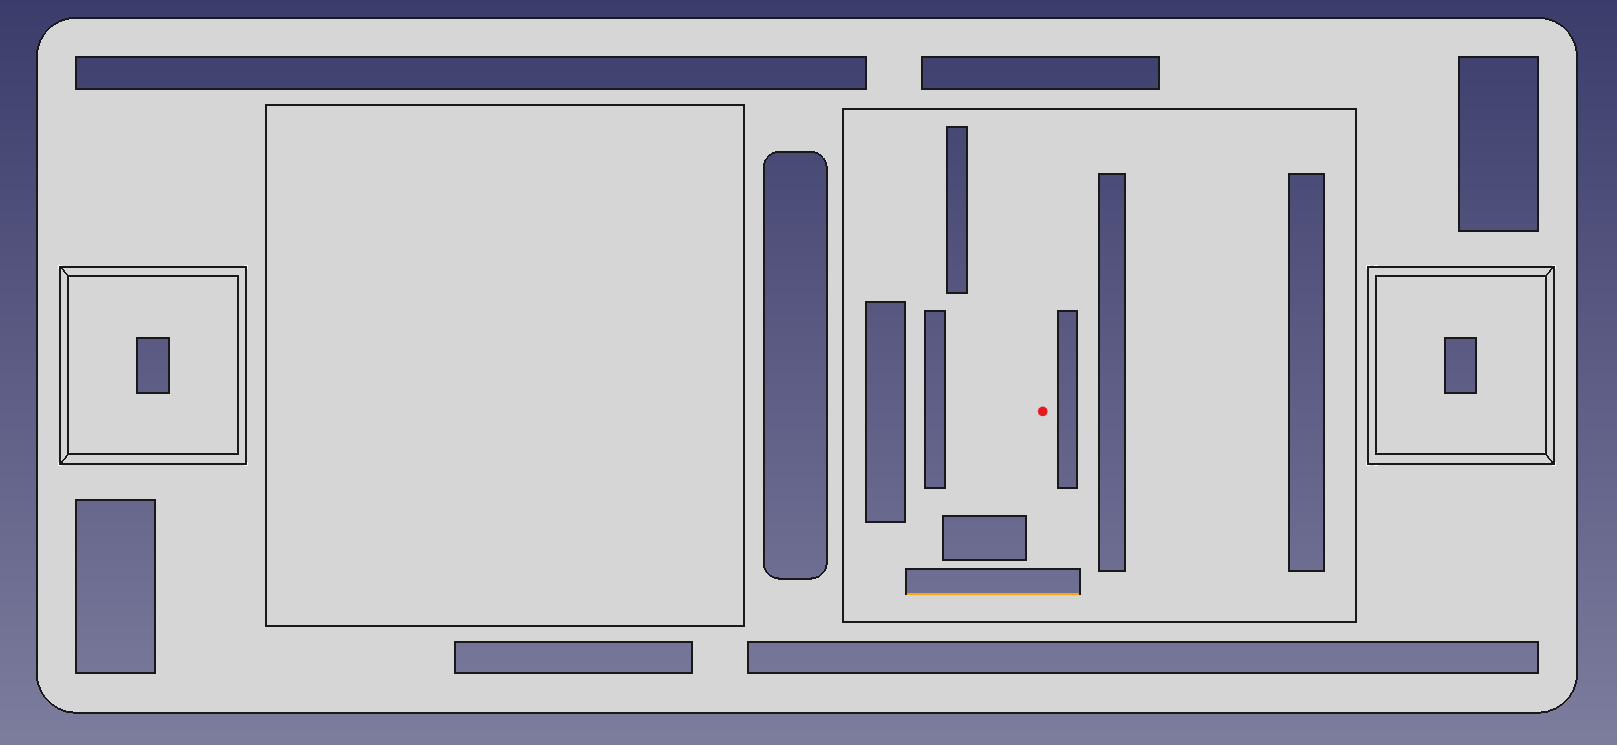
\includegraphics[width=1\linewidth]{Base}
 	\caption{}
 	\label{fig:base}
 \end{figure}
 
 \section{Software}
 Para cargar nuestros programas en el microcontrolador utilizamos el IDE de arduino, que nos servirá también para este tipo de dispositivos. Para que todo funcione debemos descargarnos mediante el gestor de tarjetas el modelo de esp32 para que nuestro ordenador lo reconozca correctamente. Además, debemos descargarnos un pequeño paquete de software de windows desde el gestor de dispositivos para que haya una comunicación efectiva entre Windows y el esp32. Por otro lado debemos descargarnos la librería del sensor, que es la que nos permitirá la comunicación I2C. 
 \paragraph{}
 Con todas nuestras extensiones instaladas debemos implementar el control PID y calibrarlo de manera correcta para que nuestro péndulo oscile lo menos posible. La cantidad de corriente que le daremos a nuestros motores la decidirá la posición del giroscopio, de esta forma nos aproximaremos más rápidamente a la posición deseada cuanto más lejos estemos de ella. Esta variación de corriente es posible gracias a los pines PWM que van del micro hasta el driver. 
  \paragraph{}
  Lo primero que debemos hacer es calibrar la posición desde la que va a trabajar nuestro sensor. Después de esto calibraremos nuestro control PID, primero ajustando \textbf{$K_p$}, después  \textbf{$K_i$}, y por último \textbf{$K_d$}. En nuestro caso no utilizaremos esta última constante ya que no mejorará en absoluto el control del péndulo. 
  \paragraph{}
  
  Cuando conseguimos que el péndulo se volviese estable tras aplicarle diversas fuerzas para intentar que se cayese comenzamos el proceso para añadir la opción de controlar el dispositivo desde una dirección IP desde cualquier buscador. Para ello es muy útil el módulo Wi-fi del microcontrolador ya que nos permite establecer el dispositivo como master de una red inalámbrica propia. Empleando esta red y usando lenguaje html para crear la página desde la que controlamos el dispositivo ya podemos moverlo como tal, así como apagarlo y encenderlo.
  {\normalsize }
\end{document}
